% !TEX root = ../thesis.tex


\chapter{Theoretical Background}
\label{cha:eva_theory}
In this chapter, I will present the theory behind evaporative cooling and the simulation of gas dynamics in a rarefied atomic gas.

I will first explain the concept of evaporative cooling in an arbitrary power law potential, including the conditions that need to be reached to achieve efficient evaporation. In the second section, I will describe the general problem of a molecular dynamics simulation and the simulation method used in this work.

\section{Theory of Evaporative Cooling}
\label{sec:evaporative_cooling_theory}
Evaporative cooling is a method to reach temperatures below the recoil limit as well as high phase space densities, which is a requirement for the onset of Bose-Einstein condensation~\cite{pethick_smith_2008}. The concept of evaporative cooling is illustrated in Figure~\ref{fig:evaporative_cooling_sketch}. A gas of atoms with temperature $T_0$ is trapped in potential with depth $U_0$. In equilibrium, the speeds in the gas are distributed according to a Maxwell-Boltzmann distribution. If the potential depth is then lowered to $U'$, a portion of atoms with energies above $U'$ can leave the trap. The remaining atoms then thermalise to a lower temperature $T'$. 
\begin{figure}[htbp]
    \centering
    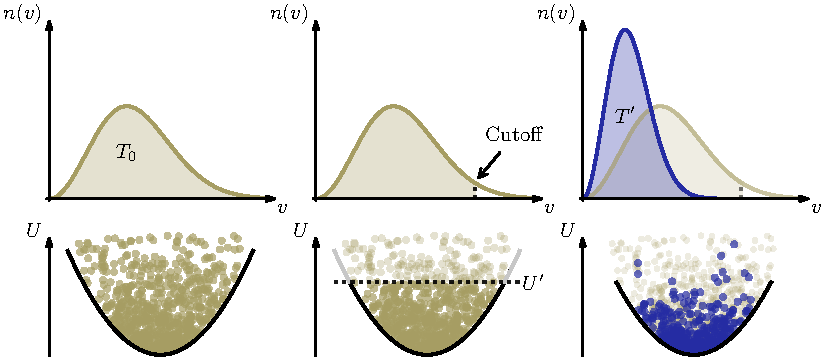
\includegraphics[]{Evap/EvaporationSketch}
    \caption{Concept of evaporative cooling}
    \label{fig:evaporative_cooling_sketch}
\end{figure}

% Many textbooks constrain themselves to a harmonic potential for a model of evaporative cooling\insertcite{}. However, as we want to simulate a box potential, I will use a generalised power-law potential to derive basic scaling laws for the evaporation process.

\subsection{The Ideal Gas in a Power-Law-Potential}
We look at an ideal gas in a general power-law-potential
%
\begin{equation*}
    U(\vec{r}) = U_x \left| \frac{x}{x_0} \right|^{\alpha_x} + U_y \left| \frac{y}{y_0} \right|^{\alpha_y} + U_z \left| \frac{z}{z_0} \right|^{\alpha_z}.
\end{equation*}
%
The density of states in such a potential has been derived in \cite{PhysRevA.35.4354} but because there is a slight error in their derivation, making it incorrect for any odd $\alpha_x$, $\alpha_y$ or $\alpha_z$, the complete and correct derivation is presented in the appendix under \ref{sec:appendix_dos}. The result is
%
\begin{equation*} %\label{eq:general_dos}
    D(E) = \left(\frac{2m}{\pi\hbar^2}\right)^\frac{3}{2} \frac{x_0 y_0 z_0}{U_x^{1/\alpha_x} U_y^{1/\alpha_y} U_z^{1/\alpha_z}} \frac{F(\alpha_x,\alpha_y,\alpha_z)}{\Gamma(\xi)} \times E^{\xi - 1}
\end{equation*}
with
\begin{equation*}
    \xi = \frac{3}{2} + \frac{1}{\alpha_x} + \frac{1}{\alpha_y} + \frac{1}{\alpha_z} \quad \text{and} \quad F(\alpha_x, \alpha_y, \alpha_z) = \prod_{i \in \{x,y,z\}} \Gamma\!\left(1 + \frac{1}{\alpha_i}\right).
\end{equation*}
%
From the density of states, we can calculate the partition function $Z$ as
\begin{align*}
    Z &= \int_0^\infty D(E)\exp{\!\left(-\frac{E}{\kB T}\right)} \diff{E} \nonumber \\
      &= \left(\frac{2m}{\pi\hbar^2}\right)^\frac{3}{2} \frac{x_0 y_0 z_0}{U_x^{1/\alpha_x} U_y^{1/\alpha_y} U_z^{1/\alpha_z}} F(\alpha_x, \alpha_y, \alpha_z) \times (\kB T)^\xi \label{eq:partition_function}
\end{align*}
and using \cite{laurendeau_2005}
\begin{equation}
    U = -N \frac{\partial \ln Z}{\partial \beta} \quad \text{with} \quad \beta = \frac{1}{\kB T} \nonumber
\end{equation}
we can write down the internal energy $U$:
\begin{equation*}
    U = N \xi \kB T.
\end{equation*}
This is consistent with the well known results of $U = 3N\kB T$ for the harmonic oscillator potential and $U = \frac{3}{2} N \kB T$ for the 3D box potential.

Furthermore, we can calculate both the spatial density and the momentum distribution by integrating out parts of the phase space distribution function
\begin{equation*}
    f(\vec{r},\vec{p}) = Z^{-1}\exp\!{\left(-\frac{\frac{\vec{p}^2}{2m} + U(\vec{r})}{\kB T}\right)}.
\end{equation*}
Integrating out the momenta and multiplying with the atom number $N$ gives us the spatial density
\begin{align}
    n(\vec{r}) &= N\int_{-\infty}^\infty \frac{\multidiff{3}{p}}{(2\pi\hbar)^3} f(\vec{r},\vec{p}) \nonumber \\
    %
    &= 4\pi N Z^{-1} (2\pi\hbar)^{-3} \int_0^\infty \diff{p}\, p^2 \exp\!\left(-\frac{\frac{\vec{p}^2}{2m} + U(\vec{r})}{\kB T}\right) \nonumber \\
    %
    &= N \left(\frac{m\kB T}{2\pi\hbar^2}\right)^{\frac{3}{2}} Z^{-1} \exp\!\left(-\frac{U(\vec{r})}{\kB T}\right) \nonumber \\
    %
    &= \underbrace{\underbrace{\frac{N}{8x_0y_0z_0}}_{=n_\text{Box}}\frac{1}{F(\alpha_x\alpha_y\alpha_z)}\prod_{i\in\{x,y,z\}}\left(\frac{U_i}{\kB T}\right)^{\frac{1}{\alpha_i}}}_{\equiv\, n_0} \exp\!\left(-\frac{U(\vec{r})}{\kB T}\right) \label{eq:spatial_density}
\end{align}
where we have defined the peak density $n_0$. In the case of a 3D box potential where $\alpha_x = \alpha_y = \alpha_z \rightarrow \infty$, the density is constant and given by $n_\text{Box} = \frac{N}{8x_0y_0z_0}$.
For future reference, we also want to calculate the average density $\bar{n}$ here. The average of any quantity $Q$ over a given density distribution $n(\vec{r})$ is given by
\[\overline{Q} = \frac{\int_{-\infty}^\infty \multidiff{3}{r}\; Q n(\vec{r})}{\int_{-\infty}^\infty \multidiff{3}{r}\; n(\vec{r})} = \frac{1}{N} \int_{-\infty}^\infty \multidiff{3}{r}\; Q n(\vec{r})\]
so for the average density we put
\begin{align}
    \bar{n} &= \frac{1}{N} \int_{-\infty}^{\infty} \multidiff{3}{r} \left(n(\vec{r})\right)^2 \nonumber \\
    &= \frac{N}{(8x_0y_0z_0)^2} \frac{1}{\left(F(\alpha_x,\alpha_y,\alpha_z)\right)^2} \left(\prod_{i\in\{x,y,z\}} \left(\frac{U_i}{\kB T}\right)^{\frac{1}{\alpha_i}} \right)^2 \int_{-\infty}^{\infty} \multidiff{3}{r} \exp\!\left(-\frac{2U(\vec{r})}{\kB T}\right) \nonumber \\
    &= \frac{N}{(8x_0y_0z_0)^2} \frac{1}{\left(F(\alpha_x,\alpha_y,\alpha_z)\right)^2} \left(\prod_{i\in\{x,y,z\}} \left(\frac{U_i}{\kB T}\right)^{\frac{1}{\alpha_i}} \right)^2 \nonumber \\
    &\phantom{=} \times 8x_0y_0z_0 \prod_{i\in\{x,y,z\}} \left(\frac{\kB T}{2 U_i}\right)^{\frac{1}{\alpha_i}} F(\alpha_x,\alpha_y,\alpha_z) \\
    &= \frac{N}{8x_0y_0z_0} \frac{2^{\frac{3}{2} - \xi}}{F(\alpha_x,\alpha_y,\alpha_z)} \prod_{i\in\{x,y,z\}} \left(\frac{U_i}{\kB T}\right)^{\frac{1}{\alpha_i}} \nonumber \\
    &= \frac{1}{2^{\xi - \frac{3}{2}}} n_0 \label{eq:mean_density}
\end{align}
For example, in the harmonic oscillator potential, this is $\bar{n} = \frac{n_0}{\sqrt{8}}$.

\pagebreak
\noindent
Similarly, we obtain the momentum distribution by integrating out the spatial coordinates:
\begin{align}
    n(\vec{p}) &= Z^{-1} \left[\int_{-\infty}^\infty \frac{\multidiff{3}{r}}{(2\pi\hbar)^3} \exp\!\left(-\frac{U(\vec{r})}{\kB T}\right) \right]\exp\!\left(-\frac{\vec{p}^2}{2m\kB T}\right)\nonumber \\
    %
    &= \frac{8x_0y_0z_0}{Z(2\pi\hbar)^3} \prod_{i\in\{x,y,z\}} \left(\frac{\kB T}{U_i}\right)^{\frac{1}{\alpha_i}} F(\alpha_x,\alpha_y,\alpha_z) \exp\!\left(-\frac{\vec{p}^2}{2m\kB T}\right) \nonumber \\
    %
    &= \frac{1}{(2\pi m \kB T)^\frac{3}{2}} \exp\!\left(-\frac{\vec{p}^2}{2m\kB T}\right) \nonumber
\end{align}
recovering the Maxwell-Boltzmann distribution.
From this, the mean speed $\overline{c}$ follows as
\begin{equation}
    \overline{c} = \frac{\langle |\vec{p}| \rangle}{m} = \frac{1}{m}\int \multidiff{3}{p} |\vec{p}|n(\vec{p}) = \sqrt{\frac{8\kB T}{\pi m}}.
\end{equation}

\subsection{Model for Evaporative Cooling}
Following the simple model explained above, we describe evaporative cooling as a sequence of infinitesimal steps in which a number \diff{N} of atoms is removed from the cloud by reducing the trap depth to a value $\eta \kB T$. Evaporative cooling is described for example in \cite{KETTERLE1996181}. Assuming $\eta \gg 1$, the loss in internal energy can be approximated as
\begin{equation}
    \diff{U} \simeq \eta \kB T \diff{N}
\end{equation}
which reduces the temperature after thermalisation by \diff{T} and the internal energy to the final value
\begin{equation}
    U_\text{f} = \xi (N - \diff{N}) \kB (T - \diff{T}).
\end{equation}
By subtracting the change in internal energy from the initial value $U_\text{i}$, we can get a relation between the change in atom number and the change in temperature:
\begin{align}
    U_\text{i} - \diff{U} &= U_\text{f} \nonumber \\
    \xi N \kB T - \eta \kB T \diff{N} &= \xi (N - \diff{N}) \kB (T - \diff{T}) \nonumber \\
    &\simeq \xi (TN - N\diff{T} - T\diff{N})\kB \nonumber
\end{align}
omitting second order terms in \diff{T} and \diff{N}.
This can be reduced to
\begin{equation*}
    \frac{\frac{\diff{T}}{T}}{\frac{\diff{N}}{N}} = \frac{\diff{\ln T}}{\diff{\ln N}} = \frac{\eta}{\xi} -1 \equiv \nu
\end{equation*}
where we define the parameter $\nu$. Trivially, for certain starting conditions $N_0$ and $T_0$ we get
\begin{equation*}
    \frac{T}{T_0} = \left(\frac{N}{N_0}\right) ^\nu.
\end{equation*}
Because the goal of evaporative cooling is to reach quantum degeneracy, cooling alone is not enough. It is also necessary to increase the phase space density \PSD which is given by
\begin{align}
    \PSD &= n_0(N,T)\cdot \left(\lambdadB(T)\right)^3 \nonumber
    \intertext{with the de-Broglie wavelength}
    \lambdadB &= \sqrt{\frac{2\pi\hbar^2}{m\kB T}}. \nonumber
\end{align}
Plugging in our result for $n_0$ from \eqref{eq:spatial_density} and the scaling of temperature with atom number, we find
\begin{equation*}
    \PSD \propto NT^{-\left(\xi - \frac{3}{2}\right)} \cdot T^{-\frac{3}{2}} \propto N^{1 - \xi\nu} = N^{1 + \xi - \eta}.
\end{equation*}
The decrease in temperature is achieved by thermalisation, which relies on elastic collisions. In an ideal gas, the elastic collision rate \Rcoll is given by \cite[8]{bird1994}
\[
   \Rcoll = n \meanProb
\]
where $n$ is the density and \meanProb the ensamble average of the product of cross section and relative velocity. As we are dealing with low temperatures, only $s$-wave scattering needs to be considered \cite{joachain}. For this simple model, we also set the cross section to be constant. The mean relative speed is proportional to the mean speed. Inserting our result for the mean density from above, we find
\begin{align}
    \overline{\Rcoll} &= \overline{n}\cdot \meanProb = \overline{n} \sigma \langle\crel\rangle \nonumber \\
    &\propto NT^{-\left(\xi - \frac{3}{2}\right)} \cdot \text{const.} \cdot T^{\frac{1}{2}} \nonumber = NT^{1-\xi} \nonumber \\
    &\propto N^{\eta \left(\frac{2}{\xi} - 1\right) + \xi - 1}. \nonumber
\end{align}

\subsubsection*{Conditions for Efficient Evaporation}
Necessary conditions to achieve evaporation are that the temperature decreases and the phase space density increases with atom number. The collision rate should at least stay constant, if it increases with atom number, \emph{runaway evaporation} occurs. As we know the scaling behaviour of these quantities with $N$, we can give the requirements for $\eta$ that have to be fulfilled to achieve each of these conditions. These are calculated in Table~\ref{tab:eva_scalings} for a linear trap (e.g.\ quadrupole trap, $\xi = 4.5$), a harmonic trap (e.g.\ Ioffe-Pritchard Trap, $\xi = 3$) and a box trap ($\xi = 1.5$).
\begin{table}[htbp]
    \centering
    \begin{tabular}{lcccl}
        \toprule
        Quantity & Scaling $N^{\{\ \}}$ & \multicolumn{3}{c}{Requirement for $\eta$} \\
        & & \multicolumn{1}{c}{linear} & \multicolumn{1}{c}{harmonic} & \multicolumn{1}{c}{box} \\
        \midrule 
        Temperature $T$ & $-1 + \frac{\eta}{\xi}$ & $\eta > \num{4.5}$ & $\eta > \num{3}$ & $\eta > \num{1.5}$ \\
        Phase Space Density $\PSD$ & $1 + \xi - \eta$ & $\eta > \num{5.5}$ & $\eta > \num{4}$ & $\eta > \num{2.5}$ \\
        Collision Rate \Rcoll & $\xi - 1 + \eta\left(\frac{2}{\xi} - 1\right)$ & $\eta > \num{6.3}$ & $\eta > \num{6}$ & $\eta < \num{-1.5}$ \\
        \bottomrule
    \end{tabular}
    \caption{Scaling laws and requirements for the parameter $\eta$ to achieve (runaway) evaporation}
    \label{tab:eva_scalings}
\end{table}
As we can see, efficient evaporation in a stationary box potential cannot be achieved. This result is very intuitive as the local density is independent of the position in this case, which means it can only decrease with a decrease in atom number. Therefore thermalisation times increase exponentially. 
This adverse interplay between density and the thermalisation rate also plays a role for other trapping configurations and several papers have been published about methods to circumvent this problem in optical dipole traps (dimple trap \cite{Jacob_2011}, tilted trap \cite{PhysRevA.78.011604, PhysRevA.79.061406}, crossed beam trap \cite{ARNOLD20113288}, zoom lenses \cite{PhysRevA.71.011602}).

% Our concept, as explained in chapter~\ref{char:eva_motivation} is a very similar ansatz, but for a box potential instead.
% It should be immediately obvious that evaporative cooling in a box potential is not something that could be meaningfully pursued. However, all the previous considerations assumed that the parameters $U_{\{x,y,z\}}$ and $x_0,y_0,z_0$ stay constant during the evaporation trajectory. If the volume of a hypothetical box potential could shrink while evaporation is performed, the adverse effect of the decreasing density could be conquered. Similar\insertcite{}, concepts have been developed and are frequently implemented with optical evaporation, where two traps with different confinement overlap or where zoom lenses are used to compress the atomic cloud during the cooling stage. 

\subsection{Inelastic Atom Loss}
Up until now we only considered elastic collisions between atoms from the cold cloud, because these are the driving mechanism behind evaporative cooling. Elastic collisions with the background gas as well as inelastic collisions between the atoms however are detrimental to the cooling effect. Atoms removed through these are not exclusively from the high-temperature end of the Maxwell-Boltzmann distribution. Even more, because inelastic losses occur through density dependent effects, in traps with non-uniform density distributions, atoms are more likely to be lost from high-density regions where cold atoms are usually accumulated. 

\subsubsection*{Background Collisions}
Collisions with the background gas in the vacuum chamber lead to atom loss because the background atoms (being in equilibrium with the walls of the chamber) are usually at room temperature (\SI{300}{K}), which means that a collision often imparts more kinetic energy onto the trapped atom than the trap depth. The collision rate with the background gas atoms is calculated via
\begin{equation*}
    \Gamma_\text{BG} = \sum_i n_i \langle \sigma v \rangle_{X,i} 
\end{equation*}
where the $i$ represent the different atomic species present in the background gas and $X$ is the trapped atomic species. The densities are related to the partial pressures by
\begin{equation}
    n_i = \frac{P_i}{\kB T} \nonumber
\end{equation}
and for ultracold atoms, the background loss rate is simply the trap lifetime at low density \cite{PhysRevLett.91.123201}.

\subsubsection*{Two-Body Collisions -- Spin Relaxation} 
Collisions of two trapped atoms can only be inelastic if the spin projections of the involved atoms change during the collisions. 
%For example, if two $^{87}$Rb atoms in the $|F=2,m_F=2\rangle$ state collide, the outgoing atoms can depart with different spin quantum numbers \cite{mies1996}. 
This process is called spin relaxation and in magnetic traps, one of the departing states can be untrapped. However, these kinds of processes can usually be suppressed by preparing the atomic cloud in a stretched spin state \cite{PhysRevLett.99.223201}.

\subsubsection*{Three-Body Collisions -- Molecule Formation}
The final process we include is the three-body collision, where two atoms form a bound state and transfer the binding energy and momentum difference to a third atom \cite{PhysRevLett.91.123201}. Usually, this leads to all three atoms being lost from the trap.

The loss rate for three-body recombination depends roughly on the square of the local density as three atoms need to be present. This also means that it can often be neglected at low densities but becomes dominant at very high densities, limiting the maximum achievable density \cite{PhysRevA.85.053647}.

\subsubsection*{Loss Rate Equation}
If the rates for background ($K_1$), 2-body ($K_2$) and 3-body ($K_3$) losses are known, the local\footnote{If we wanted to describe losses for the whole sample, we would need to take the averages $\langle n\rangle$ and $\langle n^2 \rangle$ instead.} loss rate can be expressed as
\begin{align} \label{eq:lossrate}
    \frac{1}{N}\frac{\diff{N}}{\diff{t}} = - K_1 - K_2 n - K_3 n^2.
\end{align}
where $\frac{\diff{N}}{N}$ represents the probability of an individual atom to be lost in an infinitesimal timestep $\diff{t}$.



% \section{Scattering Theory}
% \todo[inline]{derive the cross section formula used later and the mean collision rate}

\section{Numerical Simulation of Gas Dynamics}
\label{sec:dsmc_theory}

Simulating evaporative cooling is, in a bigger picture, the same as simulating any gas flow. A large number $N$ of particles, atoms or molecules, move according to a set of equations, can collide with each other and may or may not have interactions with a confining potential. A parameter that decides which model is best used to describe a gas flow is the Knudsen number \Kn, the ratio of the mean free path $\lambda$ to the length scale of the surrounding environment $L$.
\begin{equation*}
    \Kn = \frac{\lambda}{L}
\end{equation*}
In our case, this would be the side length of the volume in which the atoms are confined. Based only on this ratio, gas flows can be separated roughly into four different regimes \cite{schaaf:1958}
\begin{itemize}
    \item $\Kn < \num{.01}$: Continuum regime
    \item $\num{.01} < \Kn < \num{.1}$: Slip regime
    \item $\num{.1} < \Kn < \num{10}$: Transition regime
    \item $\Kn > 10$: Free molecular flow
\end{itemize}
Ultracold atomic gases, as they are present during evaporative cooling, usually exhibit a high Knudsen number. For example, a gas of $^{87}$Rb (scattering length $a\sim 100 a_0$ \cite{PhysRevA.87.053614}) atoms confined in a box with a side length of \SI{2}{mm} with a density of \SI{e11}{\per\centi\meter\cubed} would have a Knudsen number of $\Kn = \num{7.1}$. For this calculation, a constant cross section $\sigma = 8\pi a^2$ was assumed, which is justified at low temperatures. The more correct $s$-wave scattering cross section for identical bosons is given by \cite{dalibardCollision}
\begin{equation}  \label{eq:crosssection}
    \sigma(k) = \frac{8\pi a^2}{1 + (ak)^2} 
\end{equation}
which approaches the constant value for low collision energies. This cross section will be used in the full simulation.

We can therefore safely assume a rarefied or highly rarefied gas flow that fulfills the conditions of the transition or even free molecular regimes. The simulation method most appropriate for these regimes is the Direct Simulation Monte Carlo (DSMC) method originally developed by G.~A.~Bird \cite{bird1994}.
% In a very simple, but near complete model, interparticle dynamics are described as forces acting between the particles. This gives the complete force $\vec{F}$ acting on one particle denoted with the index $i$:
% %
% \begin{equation}
%     \vec{F}_i = -\nabla U(\vec{r}_i) + \sum_{j = 0,\, i\neq j}^N \vec{F}_{ij}
% \end{equation}
% %
% Here, $U$ is the external potential and $\vec{F}_{ij}$ is the interparticle force between particles $i$ and $j$. Naively, one could program a simulation that would calculate each of these forces at discretised timesteps and integrate the system with any differential equation solver. It is however immediately obvious why this is not feasible, at least as soon the system is a many-particle system. With ultracold gases, atom numbers $\sim$\num{E8} are not uncommon\insertcite{}. This means, there are $\sim$\num{E16} calculations necessary to get all interparticle forces, and this has to be repeated in each step. Current computer hardware is simply not powerful enough to handle extensive calculations like this. However, evaporative cooling is an example of a rarefied gas flow. The classical mean free path is given by
% \begin{equation}
%     \lambda = \frac{1}{n\sigma}
% \end{equation}
% and from, the Knudsen number $\text{Kn}$ is derived as
% \begin{equation}
%     \text{Kn} = \frac{\lambda}{L}
% \end{equation}
% where $L$ is the characteristic length scale of the medium. For an ultracold gas at typical conditions during evaporative cooling, i.e.\ a temperature of \SI{1}{\micro\kelvin}, a density of \SI{e11}{\per\cubic\centi\metre}, and a scattering length on the order of $200a_0$ that has a diameter of \SI{1}{mm}, the Knudsen number would be 
% \[\text{Kn} > 1 \]
% which puts us into the transition regime or almost into the regime of free molecular flow. When a gas is rarefied like this, numerical methods can be used to limit the computational expense necessary. Specifically, we will use the DSMC (Direct Simulation Monte Carlo) method, which is valid for Knudsen numbers $\text{Kn} > \num{0.1}$.\insertcite{MULTIPLES}


\section{The DSMC Method}
Simulating the flow of a gas with upwards of \num{e8} particles is a computational expensive task. Over a certain time $\Dt$, the probability of two particles colliding with each other is proportional to the cross section and the relative velocity. This can be imagined as the cylindrical volume that a circle with an area equal to the cross section traces out while moving with the relative velocity \cite[7]{bird1994}. As the number of possible particle pairs scales quadratically, calculating the probabilities for all pairs becomes a virtually impossible task. 

In DSMC, several measures are taken that reduce the computational expense significantly, making it possible to run a simulation on a home desktop or a laptop:
Time is discretised into small timesteps that are much smaller than the mean collision time. The simulation volume is divided into cells, each of which is treated separately for the collision handling. The number of particles in the simulation is far lower than the number of simulated particles. For the sake of better readability and because our simulation only deals with monatomic gases, a particle in the real world will be described as an \emph{atom} from now on, while particles present in the simulation will be described as \emph{particles}. A particle in the simulation represents a certain number of atoms in the real world. This number is called the statistic weight $W$ and plays an important role in the collision handling. Over one timestep, the particle movement is uncoupled from the collisions. The process of a DSMC simulation is sketched in Figure~\ref{fig:dsmc_flowchart}. The following subsections will go into more detail on each of the steps.
\begin{figure}[htbp]
    \centering
    \usetikzlibrary{positioning,calc,math,arrows}
\tikzset{mynode/.style={rectangle,rounded corners,draw=gray,inner sep=9pt,line width=0.6pt}}
\tikzset{arr/.style={-latex,color=green!25!gray}}
\tikzset{arr/.style={-latex,color=progression1}}
\begin{tikzpicture}
    \node[] (start) at (0,0) {Start};
    \tikzmath{\D=0.6;}
    \node[mynode,below=\D cm of start] (init) {\parbox{2.6cm}{\centering Initialisation {\footnotesize {Particle creation}}}};

    \node[mynode,below=\D cm of init] (move) {\parbox{3.5cm}{\centering Move particles {\footnotesize {Energy Conversation}}}};

    \node[mynode,below=\D cm of move] (bound) {\parbox{3.8cm}{\centering Boundary conditions}};% {\footnotesize {Evaporation}}}};

    % \node[mynode,below=\D cm of move] (update) {\parbox{3cm}{\centering Parameter updates {\footnotesize {Potentials etc.}}}};

    % \node[mynode,below=\D cm of update] (index) {\footnotesize Cell Indexing};
    % \node[mynode,below=-0.15cm of index,fill=white] (losses) {Inelastic losses};

    \node[mynode,below=\D cm of bound] (index2) {\footnotesize Cell Indexing};
    \node[mynode,below=-0.15cm of index2,fill=white] (coll) {\parbox{3.5cm}{\centering Collision sampling {\footnotesize {Calculate new timestep}}}};

    \node[mynode,below=\D cm of coll] (output) {\parbox{3.1cm}{\centering Output physical properties}}; %{\footnotesize {$V,T,\tilde{\rho}$ \dots}}}};

    \node[mynode,below=\D cm of output] (stop) {\parbox{4.25cm}{\centering Stop condition reached?\\ {\footnotesize {$t > t_\text{end}$?}}}}; % or $\tilde{\rho} > 1$\\ or $N < N_\text{threshold}$}}}};

    \node[below=3*\D cm of stop] (finish) {\parbox{2.2cm}{\centering {\footnotesize {Give summary}} Finish}};

    \foreach \start/\end in {%
        start/init,%
        init/move,%
        move/bound,%
        bound/index2,%
        %bound/update,%
        %update/index,%
        %losses/index2,%
        coll/output,%
        output/stop%
    }
    {
        \draw[arr] (\start) -- (\end);
    }

    \draw[arr] (stop) -- (finish) node [midway,right,color=black] {\scriptsize Yes};

    \coordinate[left=2.5cm of stop] (P1);
    \coordinate[left=2.5cm of move] (P2);

    \draw[arr] (stop) .. controls (P1) and (P2) .. (move);

    \coordinate[right=2.5cm of stop] (P3);
    \coordinate[right=2.5cm of move] (P4);

    \draw[arr,opacity=0] (stop) .. controls (P3) and (P4) .. (move);
    \node[left=0.5cm of stop] {\scriptsize No};
\end{tikzpicture}
    \caption{The process of a DSMC simulation}
    \label{fig:dsmc_flowchart}
\end{figure}


\subsection{Particle Motion}
The motion of particles in a potential is a well known problem with equally well known solutions. If every particle is treated separately, the problem reduces to
\begin{equation*}
    \ddot{\vec{r}} = -\frac{1}{m}\nabla U(\vec{r})
\end{equation*}
with known starting conditions for $\dot{\vec{r}}$ and $\vec{r}$. In many cases, a very simple method like a leapfrog etc.\ are sufficient. However, with a surrounding potential that is highly dependent on the position of the particles, more advanced methods need to be used to preserve energy as good as possible.

\subsection{Boundary Conditions}
In evaporative cooling, particle loss is an essential step. After all particles have been moved, it is checked if they have moved outside a certain boundary. If they have, they get removed from the simulation. Because the total number of atoms usually decreases by a few orders of magnitude during evaporation, after some time a large number of particles would be lost from the simulation. However, the number of particles in a collisional cell should stay above a certain threshold for accurate collision numbers \cite{SUN20111}. To circumvent this problem, we impose a threshold on the number of simulated particles $N$. Once this threshold is reached, all particles still present are copied and the statistic weight is halved. Of course, this means that we have to start with a certain power of 2 as the statistic weight. To copy the particles, the $x$ and $y$ values of their position and velocity are mirrored across the origin and the $z$ value is kept the same. This imposes the restriction on the surrounding potential that it has to be conforming to this symmetry. The $z$ values are explicitly not mirrored to retain the possibility of having gravity as a potential in the simulation.

\subsection{Collisions}
\label{sec:eva_theory_collisions}
In each collision step, a number of particle pairs is calculated in every cell, given by
\begin{equation} \label{eq:ntc_npairs}
    N_\text{pairs} = \frac{1}{V_C} N_C \overline{N_C} \maxProb \Dt
\end{equation}
where $V_C$ is the volume of one cell, $N_C$ is the instantaneous number of particles in this cell, $\overline{N_C}$ is the corresponding time averaged value and \maxProb is the maximum value of the product of cross section and relative velocity over all particle pairs. 
Then, $N_\text{pairs}$ particle pairs are chosen randomly from the cell and a collision between them is performed if 
\begin{equation} \label{eq:ntc_fraction}
    \frac{\sigma \crel}{\maxProb} > R
\end{equation} 
where $R$ is a random number between 0 and 1.
The reader might now find that this is still very inefficient as \maxProb would need to be calculated by looping over all possible particle pairs. However, because the number of pairs is proportional to \maxProb and the probability is antiproportional to it, it suffices to calculate (or even guess) \maxProb only once at the beginning. If a higher value is encountered subsequently, it can be updated. Even more, the true value of the maximum for $\sigma \crel$ is only a lower bound for the \maxProb parameter. In our simulation, we will prefer better statistics by artificially increasing the number of pairs chosen through a higher than necessary value of \maxProb.

\subsubsection*{Transient Adaptive Subcell Technique}
To enforce near neighbor collisions, every cell is even further subdivided into subcells during every step. This technique has been described in \cite{SU20101136}. When a particle pair is chosen for a collision attempt, the first particle is chosen from the whole cell. If the subcell with this particle contains other particles, the collision partner is chosen from the same subcell. Otherwise, subcells are gradually searched outwards to select a viable collision partner. We also perform collision tracking meaning that a particle $j$ is not viable for a collision with particle $i$ if $i$ and $j$ have been each other's last collision partner.

This technique is called transient, because the subcell division happens locally in each step and adaptive, because the number of subcells is chosen such that each subcell contains a certain number of particles on average. In practice, we aim for maximum 2 particles per subcell. This means that the total number of subcells in $x$, $y$ and $z$ direction is given by
\begin{equation} \label{eq:tas_ncells}
    N_i = \floor{\sqrt[3]{N_C / 2}} + 1
\end{equation}
In almost all cases, this means there are less than 2 particles in each subcell.

\subsubsection*{Calculation of the Post-Collision Velocities}
It has been mentioned before that only $s$-wave scattering is considered. Therefore the collisions are isotropic and the Post-Collision Velocities are straightforward. The relative speed of the two particles does not change, only the direction of the relative velocity.
The centre-of-mass $\vec{c}_\text{COM}$ and relative velocity $\vec{c}_\text{r}$ before the collision are given by
\begin{equation*}
    \vec{c}_\text{COM} = \frac{1}{2}(\vec{c}_1 + \vec{c}_2), \quad \vec{c}_\text{r} = \vec{c}_1 - \vec{c}_2.
\end{equation*}
We calculate a unit vector of random direction as
\begin{equation*}
    \hat{\vec{R}} = \begin{pmatrix}
        \cos(\theta) \\ \sin(\theta) \cos(\phi) \\ \sin(\theta) \sin(\phi)
    \end{pmatrix}
\end{equation*}
where $\phi$ is randomly picked between $0$ and $2\pi$ and $\cos(\theta)$ is randomly picked between $-1$ and $1$.
Then the post collision velocities $\vec{c}_1'$ and $\vec{c}_2'$ are simply
\begin{equation*}
    \vec{c}_1' = \vec{c}_\text{COM} + \frac{1}{2} \crel \cdot \hat{\vec{R}}, \quad \vec{c}_2' = \vec{c}_\text{COM} - \frac{1}{2} \crel \cdot \hat{\vec{R}}.
\end{equation*}
where \crel is the absolute value of $\vec{c}_\text{r}$.


% One possible approach in order to reduce the computational complexity of the task at hand is to decouple the particle motion from the collisions over a small timestep, i.e.\ calculating and applying the motion first and then handling the collisions in a separate step. To get accurate collision numbers, the domain of the simulaion is separated into smaller cells such that in each cell, a constant density can be assumed. The size of the cells also needs to be smaller than the local mean free path\insertcite{}. With a sufficiently small timestep only near neighbor collisions, i.e.\ collisions inside the same cell, are possible. Then, the probability of a collision between two particles is given by
% %
% \begin{equation}
%     P = \sigma \crel \Dt / \Vcell.
% \end{equation}
% %
% Here, $\sigma$ is the collisional cross-section, \crel the relative speed of the particles and \Vcell the volume of the cell. One could then compute the expected number of collisions in one timestep from the collision rate, choose particle pairs at random and evaluate collisions between them based on an acceptance-rejection method. This involves choosing a random number and accepting a collision if the probability $P$ exceeds this random number and rejecting it if it does not. This approach brings the problem that $P$ is usually a very small quantity, meaning a very large number of pairs would have to be tested for collisions in each step to reach the expected collision numbers. 



% G.~A.~Bird first proposed and developed many of the algorithms that this work is based on\insertcite{}. In his \enquote{No-Time-Counter} (NTC) method, the problem mentioned above is solved the following way: A number of particle pairs is selected from each cell and the collisions are then sampled among them. Specifically,
% %
% \begin{equation} \label{eq:ntc_npairs_incomplete}
%     \frac{1}{2\Vcell} N (N - 1) \maxProb \Dt
% \end{equation}
% %
% pairs are chosen. Here, $N$ is the number of particles in the cell and \maxProb represents the maximum value of the product of cross-section and relative speed over all particle pairs in the cell. A collision of a pair $(ij)$ is accepted if
% %
% \begin{equation} \label{eq:ntc_fraction}
%     \frac{(\sigma\crel)_{ij}}{\maxProb} > R
% \end{equation}
% %
% with a random number $0 \leq R \leq 1$. Now the value of the deciding fraction in \eqref{eq:ntc_fraction} is much closer to 1 than if the probability $P$ had been calculated for each pair separately. This means that a lower number of pairs tested get's rejected, reducing the time necessary to complete one collision time step in one cell. The value of \maxProb also does not have to be calculated in each step which would take the benefits away again. Instead, it is calculated once in the beginning of the simulation and then subsequently updated if a larger value is encountered. 

% Up until now we are still dealing with an enormous amount of calculations if both the motion and collision processing have to be done for $\sim$\num{1e8} particles. Arguably the most important step to achieving lower computation times is to let each particle in the simulation be representative of a number of actual physical particles. The simulated particles are called \emph{macro}-particles from now on to avoid confusion. The number of particles represented by one macro-particle is called the statistic weight $W$. In simulations where the average number of particles is approximately constant over the simulated duration, this weight can be chosen almost arbitrarily\footnote{of cource, lower values for $W$ result in better statistic accuracy.}. However, in evaporative cooling, particle loss is inherent to the process. This means that we have to choose the weight as a power of $2$. If the number of macro-particles drops below a threshold during the simulation, the weight is halved and each macro-particle is duplicated. During this duplication procedure, the velocity and position are mirrored along at least one axis to make it impossible for the duplicated particles to collide with the \enquote{old} ones immediately after the duplication process. [\textbf{NOTE:} This requires the external potential to have spatial symmetry in at least one direction, otherwise potential energy would not be conserved.]
% With this technique, the behaviour of \num{E8} particles can be simulated using only e.g.\ $\sim$\num{12000} macro-particles, each with a statistic weight of $W=2^{13} = \num{8192}$. 
% With the inclusion of the statistic weight, equation \eqref{eq:ntc_npairs_incomplete} becomes
% %
% \begin{equation} \label{eq:ntc_npairs}
%     N_\text{pairs} = \frac{1}{2\Vcell} W N (N-1) \maxProb \Dt.
% \end{equation}
% %

% \paragraph{Transient Adaptive Sub-Cell Technique} ~\\
% Because the macroscopic parameters of an atomic cloud change rapidly during evaporative cooling, a fixed number of cells might not always guarantee the conditions that the cell size should be about $1/2$ - $1/3$ the local mean free path. However, the accuracy of the simulation can be maintained by introducing sub-cells \insertcite{}. In each step, every cell gets subdivided into sub-cells, such that each sub-cell contains a previously specified number of macro-particles. During the collision procedure, first collision partner is chosen from the whole cell. If the sub-cell of this contains other macro-particles, the second collision partner is chosen from the same sub-cell. Otherwise, the adjacent sub-cells are searched for a collision partner. 

% The technique is called \enquote{transient} because the sub-cells are created in every step and \enquote{adaptive} because the number of sub-cells can change between steps, depending on the number of macro-particles present.



% \subsection{Collisions}
% \label{sec:eva_theory_collisions}
% In ultracold gases, only $s$-wave collisions are possible due to the very low temperatures. This simplifies the calculation of the velocities in a particle pair after a collision significantly, as a hard-sphere model can be applied. This means that the magnitude of the relative velocity between the particles does not change during the collision, only its direction is reassigned at random. In a gas with identical atoms, the centre-of-mass velocity is simply given by
% %
% \begin{equation}
%     \cCOM = \frac{1}{2}(\vec{c}_1 + \vec{c}_2)
% \end{equation}
% %
% and the relative velocity is
% %
% \begin{equation}
%     \vec{c}_\text{rel} = \vec{c}_1 - \vec{c}_2.
% \end{equation}
% %
% The velocities after the collision are then calculated as
% %
% \begin{align}
%     \vec{c}_1^* &= \cCOM + \frac12 |\vec{c}_\text{rel}|\cdot\vec{\hat{R}} \\
%     \vec{c}_2^* &= \cCOM - \frac12 |\vec{c}_\text{rel}|\cdot\vec{\hat{R}}
% \end{align}
% %
% where $\vec{\hat{R}}$ is a unit vector of random direction.

% \iffalse
% \subsection{Summary}
% A number of particles is represented as a smaller number of macro-particles, each with a the number of particles per macro-particle as a statistic weight. The domain is divided into smaller cells for near neighbour collisions.
% In one timestep, the following steps are executed:
% \begin{enumerate}
%     \item move all particles according to the external forces.
%     \item apply boundary conditions (e.g.\ eject particles that have moved outside of the domain).
%     \item perform collisions in each cell seperately according to the scheme described above.
% \end{enumerate}
% \fi


